% Created by tikzDevice version 0.6.2-92-0ad2792 on 2013-03-04 16:59:18
% !TEX encoding = UTF-8 Unicode
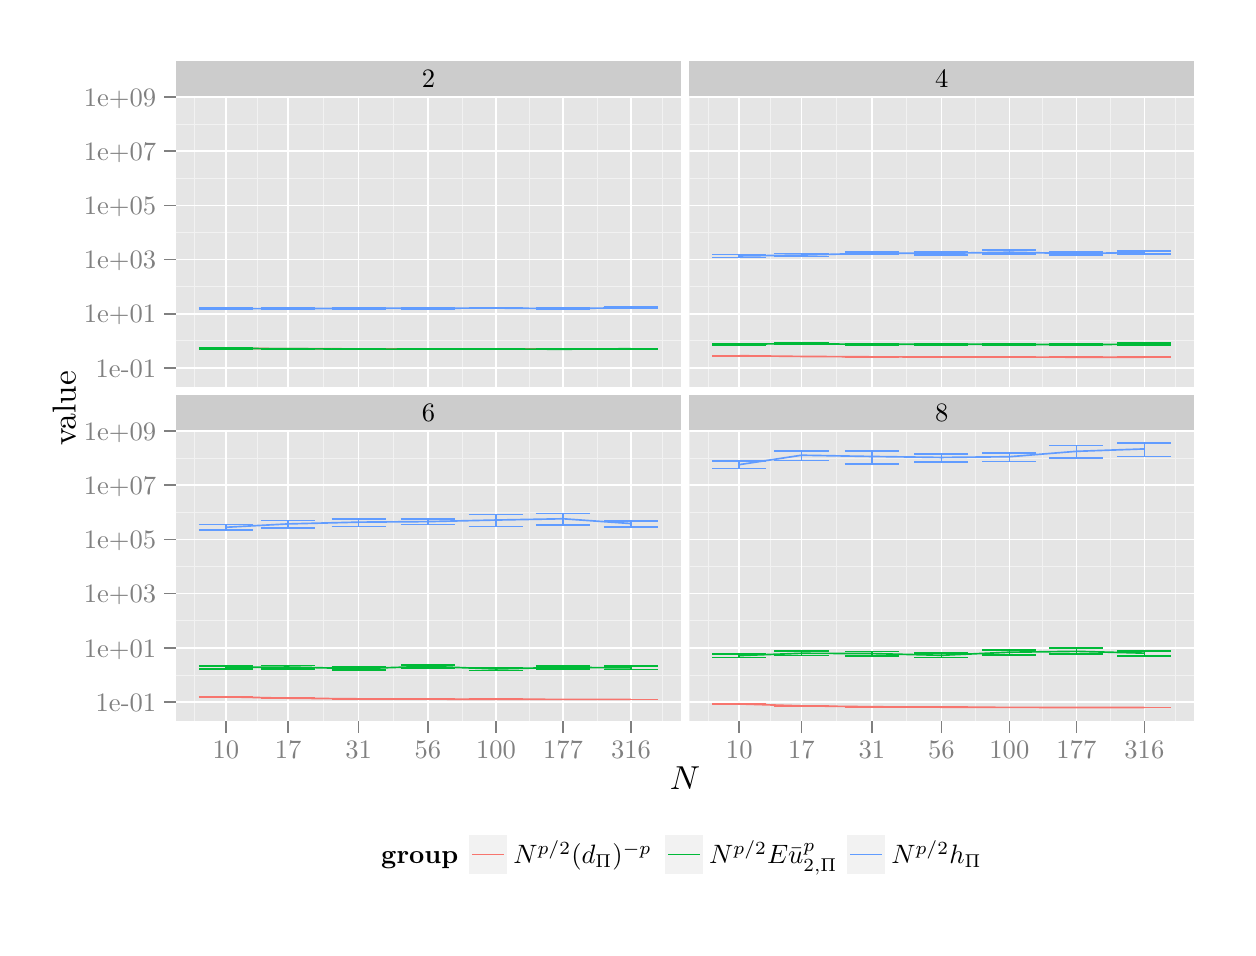
\begin{tikzpicture}[x=1pt,y=1pt]
\definecolor[named]{fillColor}{rgb}{1.00,1.00,1.00}
\path[use as bounding box,fill=fillColor,fill opacity=0.00] (0,0) rectangle (433.62,325.21);
\begin{scope}
\path[clip] (  0.00,  0.00) rectangle (433.62,325.21);
\definecolor[named]{drawColor}{rgb}{1.00,1.00,1.00}
\definecolor[named]{fillColor}{rgb}{1.00,1.00,1.00}

\path[draw=drawColor,line width= 0.6pt,line join=round,line cap=round,fill=fillColor] (  0.00,  0.00) rectangle (433.62,325.21);
\end{scope}
\begin{scope}
\path[clip] ( 53.55,195.47) rectangle (236.06,300.54);
\definecolor[named]{fillColor}{rgb}{0.90,0.90,0.90}

\path[fill=fillColor] ( 53.55,195.47) rectangle (236.06,300.54);
\definecolor[named]{drawColor}{rgb}{0.95,0.95,0.95}

\path[draw=drawColor,line width= 0.3pt,line join=round] ( 53.55,212.02) --
	(236.06,212.02);

\path[draw=drawColor,line width= 0.3pt,line join=round] ( 53.55,231.61) --
	(236.06,231.61);

\path[draw=drawColor,line width= 0.3pt,line join=round] ( 53.55,251.20) --
	(236.06,251.20);

\path[draw=drawColor,line width= 0.3pt,line join=round] ( 53.55,270.80) --
	(236.06,270.80);

\path[draw=drawColor,line width= 0.3pt,line join=round] ( 53.55,290.39) --
	(236.06,290.39);

\path[draw=drawColor,line width= 0.3pt,line join=round] ( 60.36,195.47) --
	( 60.36,300.54);

\path[draw=drawColor,line width= 0.3pt,line join=round] ( 82.85,195.47) --
	( 82.85,300.54);

\path[draw=drawColor,line width= 0.3pt,line join=round] (106.84,195.47) --
	(106.84,300.54);

\path[draw=drawColor,line width= 0.3pt,line join=round] (132.11,195.47) --
	(132.11,300.54);

\path[draw=drawColor,line width= 0.3pt,line join=round] (156.93,195.47) --
	(156.93,300.54);

\path[draw=drawColor,line width= 0.3pt,line join=round] (181.33,195.47) --
	(181.33,300.54);

\path[draw=drawColor,line width= 0.3pt,line join=round] (205.71,195.47) --
	(205.71,300.54);

\path[draw=drawColor,line width= 0.3pt,line join=round] (229.25,195.47) --
	(229.25,300.54);
\definecolor[named]{drawColor}{rgb}{1.00,1.00,1.00}

\path[draw=drawColor,line width= 0.6pt,line join=round] ( 53.55,202.22) --
	(236.06,202.22);

\path[draw=drawColor,line width= 0.6pt,line join=round] ( 53.55,221.81) --
	(236.06,221.81);

\path[draw=drawColor,line width= 0.6pt,line join=round] ( 53.55,241.41) --
	(236.06,241.41);

\path[draw=drawColor,line width= 0.6pt,line join=round] ( 53.55,261.00) --
	(236.06,261.00);

\path[draw=drawColor,line width= 0.6pt,line join=round] ( 53.55,280.59) --
	(236.06,280.59);

\path[draw=drawColor,line width= 0.6pt,line join=round] ( 53.55,300.19) --
	(236.06,300.19);

\path[draw=drawColor,line width= 0.6pt,line join=round] ( 71.61,195.47) --
	( 71.61,300.54);

\path[draw=drawColor,line width= 0.6pt,line join=round] ( 94.10,195.47) --
	( 94.10,300.54);

\path[draw=drawColor,line width= 0.6pt,line join=round] (119.57,195.47) --
	(119.57,300.54);

\path[draw=drawColor,line width= 0.6pt,line join=round] (144.64,195.47) --
	(144.64,300.54);

\path[draw=drawColor,line width= 0.6pt,line join=round] (169.22,195.47) --
	(169.22,300.54);

\path[draw=drawColor,line width= 0.6pt,line join=round] (193.43,195.47) --
	(193.43,300.54);

\path[draw=drawColor,line width= 0.6pt,line join=round] (218.00,195.47) --
	(218.00,300.54);
\definecolor[named]{drawColor}{rgb}{0.97,0.46,0.43}

\path[draw=drawColor,line width= 0.6pt,line join=round] ( 71.61,209.33) --
	( 94.10,209.21) --
	(119.57,209.14) --
	(144.64,209.11) --
	(169.22,209.09) --
	(193.43,209.08) --
	(218.00,209.07);
\definecolor[named]{drawColor}{rgb}{0.00,0.73,0.22}

\path[draw=drawColor,line width= 0.6pt,line join=round] ( 71.61,209.30) --
	( 94.10,209.20) --
	(119.57,209.05) --
	(144.64,209.08) --
	(169.22,209.11) --
	(193.43,209.01) --
	(218.00,209.19);
\definecolor[named]{drawColor}{rgb}{0.38,0.61,1.00}

\path[draw=drawColor,line width= 0.6pt,line join=round] ( 71.61,223.69) --
	( 94.10,223.69) --
	(119.57,223.78) --
	(144.64,223.83) --
	(169.22,223.87) --
	(193.43,223.71) --
	(218.00,224.00);
\definecolor[named]{drawColor}{rgb}{0.97,0.46,0.43}

\path[draw=drawColor,line width= 0.6pt,line join=round] ( 61.85,209.34) --
	( 81.37,209.34);

\path[draw=drawColor,line width= 0.6pt,line join=round] ( 71.61,209.34) --
	( 71.61,209.32);

\path[draw=drawColor,line width= 0.6pt,line join=round] ( 61.85,209.32) --
	( 81.37,209.32);

\path[draw=drawColor,line width= 0.6pt,line join=round] ( 84.34,209.21) --
	(103.86,209.21);

\path[draw=drawColor,line width= 0.6pt,line join=round] ( 94.10,209.21) --
	( 94.10,209.20);

\path[draw=drawColor,line width= 0.6pt,line join=round] ( 84.34,209.20) --
	(103.86,209.20);

\path[draw=drawColor,line width= 0.6pt,line join=round] (109.81,209.14) --
	(129.33,209.14);

\path[draw=drawColor,line width= 0.6pt,line join=round] (119.57,209.14) --
	(119.57,209.14);

\path[draw=drawColor,line width= 0.6pt,line join=round] (109.81,209.14) --
	(129.33,209.14);

\path[draw=drawColor,line width= 0.6pt,line join=round] (134.88,209.11) --
	(154.40,209.11);

\path[draw=drawColor,line width= 0.6pt,line join=round] (144.64,209.11) --
	(144.64,209.11);

\path[draw=drawColor,line width= 0.6pt,line join=round] (134.88,209.11) --
	(154.40,209.11);

\path[draw=drawColor,line width= 0.6pt,line join=round] (159.46,209.09) --
	(178.98,209.09);

\path[draw=drawColor,line width= 0.6pt,line join=round] (169.22,209.09) --
	(169.22,209.09);

\path[draw=drawColor,line width= 0.6pt,line join=round] (159.46,209.09) --
	(178.98,209.09);

\path[draw=drawColor,line width= 0.6pt,line join=round] (183.67,209.08) --
	(203.19,209.08);

\path[draw=drawColor,line width= 0.6pt,line join=round] (193.43,209.08) --
	(193.43,209.08);

\path[draw=drawColor,line width= 0.6pt,line join=round] (183.67,209.08) --
	(203.19,209.08);

\path[draw=drawColor,line width= 0.6pt,line join=round] (208.24,209.07) --
	(227.76,209.07);

\path[draw=drawColor,line width= 0.6pt,line join=round] (218.00,209.07) --
	(218.00,209.07);

\path[draw=drawColor,line width= 0.6pt,line join=round] (208.24,209.07) --
	(227.76,209.07);
\definecolor[named]{drawColor}{rgb}{0.00,0.73,0.22}

\path[draw=drawColor,line width= 0.6pt,line join=round] ( 61.85,209.41) --
	( 81.37,209.41);

\path[draw=drawColor,line width= 0.6pt,line join=round] ( 71.61,209.41) --
	( 71.61,209.19);

\path[draw=drawColor,line width= 0.6pt,line join=round] ( 61.85,209.19) --
	( 81.37,209.19);

\path[draw=drawColor,line width= 0.6pt,line join=round] ( 84.34,209.33) --
	(103.86,209.33);

\path[draw=drawColor,line width= 0.6pt,line join=round] ( 94.10,209.33) --
	( 94.10,209.09);

\path[draw=drawColor,line width= 0.6pt,line join=round] ( 84.34,209.09) --
	(103.86,209.09);

\path[draw=drawColor,line width= 0.6pt,line join=round] (109.81,209.16) --
	(129.33,209.16);

\path[draw=drawColor,line width= 0.6pt,line join=round] (119.57,209.16) --
	(119.57,208.93);

\path[draw=drawColor,line width= 0.6pt,line join=round] (109.81,208.93) --
	(129.33,208.93);

\path[draw=drawColor,line width= 0.6pt,line join=round] (134.88,209.20) --
	(154.40,209.20);

\path[draw=drawColor,line width= 0.6pt,line join=round] (144.64,209.20) --
	(144.64,208.97);

\path[draw=drawColor,line width= 0.6pt,line join=round] (134.88,208.97) --
	(154.40,208.97);

\path[draw=drawColor,line width= 0.6pt,line join=round] (159.46,209.22) --
	(178.98,209.22);

\path[draw=drawColor,line width= 0.6pt,line join=round] (169.22,209.22) --
	(169.22,208.99);

\path[draw=drawColor,line width= 0.6pt,line join=round] (159.46,208.99) --
	(178.98,208.99);

\path[draw=drawColor,line width= 0.6pt,line join=round] (183.67,209.13) --
	(203.19,209.13);

\path[draw=drawColor,line width= 0.6pt,line join=round] (193.43,209.13) --
	(193.43,208.90);

\path[draw=drawColor,line width= 0.6pt,line join=round] (183.67,208.90) --
	(203.19,208.90);

\path[draw=drawColor,line width= 0.6pt,line join=round] (208.24,209.31) --
	(227.76,209.31);

\path[draw=drawColor,line width= 0.6pt,line join=round] (218.00,209.31) --
	(218.00,209.07);

\path[draw=drawColor,line width= 0.6pt,line join=round] (208.24,209.07) --
	(227.76,209.07);
\definecolor[named]{drawColor}{rgb}{0.38,0.61,1.00}

\path[draw=drawColor,line width= 0.6pt,line join=round] ( 61.85,223.87) --
	( 81.37,223.87);

\path[draw=drawColor,line width= 0.6pt,line join=round] ( 71.61,223.87) --
	( 71.61,223.51);

\path[draw=drawColor,line width= 0.6pt,line join=round] ( 61.85,223.51) --
	( 81.37,223.51);

\path[draw=drawColor,line width= 0.6pt,line join=round] ( 84.34,223.88) --
	(103.86,223.88);

\path[draw=drawColor,line width= 0.6pt,line join=round] ( 94.10,223.88) --
	( 94.10,223.49);

\path[draw=drawColor,line width= 0.6pt,line join=round] ( 84.34,223.49) --
	(103.86,223.49);

\path[draw=drawColor,line width= 0.6pt,line join=round] (109.81,223.99) --
	(129.33,223.99);

\path[draw=drawColor,line width= 0.6pt,line join=round] (119.57,223.99) --
	(119.57,223.57);

\path[draw=drawColor,line width= 0.6pt,line join=round] (109.81,223.57) --
	(129.33,223.57);

\path[draw=drawColor,line width= 0.6pt,line join=round] (134.88,224.04) --
	(154.40,224.04);

\path[draw=drawColor,line width= 0.6pt,line join=round] (144.64,224.04) --
	(144.64,223.64);

\path[draw=drawColor,line width= 0.6pt,line join=round] (134.88,223.64) --
	(154.40,223.64);

\path[draw=drawColor,line width= 0.6pt,line join=round] (159.46,224.07) --
	(178.98,224.07);

\path[draw=drawColor,line width= 0.6pt,line join=round] (169.22,224.07) --
	(169.22,223.69);

\path[draw=drawColor,line width= 0.6pt,line join=round] (159.46,223.69) --
	(178.98,223.69);

\path[draw=drawColor,line width= 0.6pt,line join=round] (183.67,223.92) --
	(203.19,223.92);

\path[draw=drawColor,line width= 0.6pt,line join=round] (193.43,223.92) --
	(193.43,223.49);

\path[draw=drawColor,line width= 0.6pt,line join=round] (183.67,223.49) --
	(203.19,223.49);

\path[draw=drawColor,line width= 0.6pt,line join=round] (208.24,224.21) --
	(227.76,224.21);

\path[draw=drawColor,line width= 0.6pt,line join=round] (218.00,224.21) --
	(218.00,223.79);

\path[draw=drawColor,line width= 0.6pt,line join=round] (208.24,223.79) --
	(227.76,223.79);
\end{scope}
\begin{scope}
\path[clip] (239.07,195.47) rectangle (421.58,300.54);
\definecolor[named]{fillColor}{rgb}{0.90,0.90,0.90}

\path[fill=fillColor] (239.07,195.47) rectangle (421.57,300.54);
\definecolor[named]{drawColor}{rgb}{0.95,0.95,0.95}

\path[draw=drawColor,line width= 0.3pt,line join=round] (239.07,212.02) --
	(421.58,212.02);

\path[draw=drawColor,line width= 0.3pt,line join=round] (239.07,231.61) --
	(421.58,231.61);

\path[draw=drawColor,line width= 0.3pt,line join=round] (239.07,251.20) --
	(421.58,251.20);

\path[draw=drawColor,line width= 0.3pt,line join=round] (239.07,270.80) --
	(421.58,270.80);

\path[draw=drawColor,line width= 0.3pt,line join=round] (239.07,290.39) --
	(421.58,290.39);

\path[draw=drawColor,line width= 0.3pt,line join=round] (245.88,195.47) --
	(245.88,300.54);

\path[draw=drawColor,line width= 0.3pt,line join=round] (268.37,195.47) --
	(268.37,300.54);

\path[draw=drawColor,line width= 0.3pt,line join=round] (292.36,195.47) --
	(292.36,300.54);

\path[draw=drawColor,line width= 0.3pt,line join=round] (317.62,195.47) --
	(317.62,300.54);

\path[draw=drawColor,line width= 0.3pt,line join=round] (342.45,195.47) --
	(342.45,300.54);

\path[draw=drawColor,line width= 0.3pt,line join=round] (366.84,195.47) --
	(366.84,300.54);

\path[draw=drawColor,line width= 0.3pt,line join=round] (391.23,195.47) --
	(391.23,300.54);

\path[draw=drawColor,line width= 0.3pt,line join=round] (414.77,195.47) --
	(414.77,300.54);
\definecolor[named]{drawColor}{rgb}{1.00,1.00,1.00}

\path[draw=drawColor,line width= 0.6pt,line join=round] (239.07,202.22) --
	(421.58,202.22);

\path[draw=drawColor,line width= 0.6pt,line join=round] (239.07,221.81) --
	(421.58,221.81);

\path[draw=drawColor,line width= 0.6pt,line join=round] (239.07,241.41) --
	(421.58,241.41);

\path[draw=drawColor,line width= 0.6pt,line join=round] (239.07,261.00) --
	(421.58,261.00);

\path[draw=drawColor,line width= 0.6pt,line join=round] (239.07,280.59) --
	(421.58,280.59);

\path[draw=drawColor,line width= 0.6pt,line join=round] (239.07,300.19) --
	(421.58,300.19);

\path[draw=drawColor,line width= 0.6pt,line join=round] (257.13,195.47) --
	(257.13,300.54);

\path[draw=drawColor,line width= 0.6pt,line join=round] (279.62,195.47) --
	(279.62,300.54);

\path[draw=drawColor,line width= 0.6pt,line join=round] (305.09,195.47) --
	(305.09,300.54);

\path[draw=drawColor,line width= 0.6pt,line join=round] (330.16,195.47) --
	(330.16,300.54);

\path[draw=drawColor,line width= 0.6pt,line join=round] (354.74,195.47) --
	(354.74,300.54);

\path[draw=drawColor,line width= 0.6pt,line join=round] (378.95,195.47) --
	(378.95,300.54);

\path[draw=drawColor,line width= 0.6pt,line join=round] (403.52,195.47) --
	(403.52,300.54);
\definecolor[named]{drawColor}{rgb}{0.97,0.46,0.43}

\path[draw=drawColor,line width= 0.6pt,line join=round] (257.13,206.67) --
	(279.62,206.41) --
	(305.09,206.26) --
	(330.16,206.20) --
	(354.74,206.16) --
	(378.95,206.14) --
	(403.52,206.13);
\definecolor[named]{drawColor}{rgb}{0.00,0.73,0.22}

\path[draw=drawColor,line width= 0.6pt,line join=round] (257.13,210.90) --
	(279.62,210.97) --
	(305.09,210.79) --
	(330.16,210.82) --
	(354.74,210.83) --
	(378.95,210.61) --
	(403.52,210.88);
\definecolor[named]{drawColor}{rgb}{0.38,0.61,1.00}

\path[draw=drawColor,line width= 0.6pt,line join=round] (257.13,242.71) --
	(279.62,243.03) --
	(305.09,243.70) --
	(330.16,243.68) --
	(354.74,244.06) --
	(378.95,243.59) --
	(403.52,243.97);
\definecolor[named]{drawColor}{rgb}{0.97,0.46,0.43}

\path[draw=drawColor,line width= 0.6pt,line join=round] (247.36,206.69) --
	(266.89,206.69);

\path[draw=drawColor,line width= 0.6pt,line join=round] (257.13,206.69) --
	(257.13,206.65);

\path[draw=drawColor,line width= 0.6pt,line join=round] (247.36,206.65) --
	(266.89,206.65);

\path[draw=drawColor,line width= 0.6pt,line join=round] (269.86,206.42) --
	(289.38,206.42);

\path[draw=drawColor,line width= 0.6pt,line join=round] (279.62,206.42) --
	(279.62,206.40);

\path[draw=drawColor,line width= 0.6pt,line join=round] (269.86,206.40) --
	(289.38,206.40);

\path[draw=drawColor,line width= 0.6pt,line join=round] (295.33,206.27) --
	(314.85,206.27);

\path[draw=drawColor,line width= 0.6pt,line join=round] (305.09,206.27) --
	(305.09,206.26);

\path[draw=drawColor,line width= 0.6pt,line join=round] (295.33,206.26) --
	(314.85,206.26);

\path[draw=drawColor,line width= 0.6pt,line join=round] (320.40,206.20) --
	(339.92,206.20);

\path[draw=drawColor,line width= 0.6pt,line join=round] (330.16,206.20) --
	(330.16,206.20);

\path[draw=drawColor,line width= 0.6pt,line join=round] (320.40,206.20) --
	(339.92,206.20);

\path[draw=drawColor,line width= 0.6pt,line join=round] (344.98,206.16) --
	(364.50,206.16);

\path[draw=drawColor,line width= 0.6pt,line join=round] (354.74,206.16) --
	(354.74,206.16);

\path[draw=drawColor,line width= 0.6pt,line join=round] (344.98,206.16) --
	(364.50,206.16);

\path[draw=drawColor,line width= 0.6pt,line join=round] (369.19,206.14) --
	(388.71,206.14);

\path[draw=drawColor,line width= 0.6pt,line join=round] (378.95,206.14) --
	(378.95,206.14);

\path[draw=drawColor,line width= 0.6pt,line join=round] (369.19,206.14) --
	(388.71,206.14);

\path[draw=drawColor,line width= 0.6pt,line join=round] (393.76,206.13) --
	(413.28,206.13);

\path[draw=drawColor,line width= 0.6pt,line join=round] (403.52,206.13) --
	(403.52,206.13);

\path[draw=drawColor,line width= 0.6pt,line join=round] (393.76,206.13) --
	(413.28,206.13);
\definecolor[named]{drawColor}{rgb}{0.00,0.73,0.22}

\path[draw=drawColor,line width= 0.6pt,line join=round] (247.36,211.12) --
	(266.89,211.12);

\path[draw=drawColor,line width= 0.6pt,line join=round] (257.13,211.12) --
	(257.13,210.66);

\path[draw=drawColor,line width= 0.6pt,line join=round] (247.36,210.66) --
	(266.89,210.66);

\path[draw=drawColor,line width= 0.6pt,line join=round] (269.86,211.21) --
	(289.38,211.21);

\path[draw=drawColor,line width= 0.6pt,line join=round] (279.62,211.21) --
	(279.62,210.70);

\path[draw=drawColor,line width= 0.6pt,line join=round] (269.86,210.70) --
	(289.38,210.70);

\path[draw=drawColor,line width= 0.6pt,line join=round] (295.33,211.04) --
	(314.85,211.04);

\path[draw=drawColor,line width= 0.6pt,line join=round] (305.09,211.04) --
	(305.09,210.51);

\path[draw=drawColor,line width= 0.6pt,line join=round] (295.33,210.51) --
	(314.85,210.51);

\path[draw=drawColor,line width= 0.6pt,line join=round] (320.40,211.08) --
	(339.92,211.08);

\path[draw=drawColor,line width= 0.6pt,line join=round] (330.16,211.08) --
	(330.16,210.57);

\path[draw=drawColor,line width= 0.6pt,line join=round] (320.40,210.57) --
	(339.92,210.57);

\path[draw=drawColor,line width= 0.6pt,line join=round] (344.98,211.09) --
	(364.50,211.09);

\path[draw=drawColor,line width= 0.6pt,line join=round] (354.74,211.09) --
	(354.74,210.57);

\path[draw=drawColor,line width= 0.6pt,line join=round] (344.98,210.57) --
	(364.50,210.57);

\path[draw=drawColor,line width= 0.6pt,line join=round] (369.19,210.89) --
	(388.71,210.89);

\path[draw=drawColor,line width= 0.6pt,line join=round] (378.95,210.89) --
	(378.95,210.32);

\path[draw=drawColor,line width= 0.6pt,line join=round] (369.19,210.32) --
	(388.71,210.32);

\path[draw=drawColor,line width= 0.6pt,line join=round] (393.76,211.15) --
	(413.28,211.15);

\path[draw=drawColor,line width= 0.6pt,line join=round] (403.52,211.15) --
	(403.52,210.62);

\path[draw=drawColor,line width= 0.6pt,line join=round] (393.76,210.62) --
	(413.28,210.62);
\definecolor[named]{drawColor}{rgb}{0.38,0.61,1.00}

\path[draw=drawColor,line width= 0.6pt,line join=round] (247.36,243.21) --
	(266.89,243.21);

\path[draw=drawColor,line width= 0.6pt,line join=round] (257.13,243.21) --
	(257.13,242.20);

\path[draw=drawColor,line width= 0.6pt,line join=round] (247.36,242.20) --
	(266.89,242.20);

\path[draw=drawColor,line width= 0.6pt,line join=round] (269.86,243.60) --
	(289.38,243.60);

\path[draw=drawColor,line width= 0.6pt,line join=round] (279.62,243.60) --
	(279.62,242.48);

\path[draw=drawColor,line width= 0.6pt,line join=round] (269.86,242.48) --
	(289.38,242.48);

\path[draw=drawColor,line width= 0.6pt,line join=round] (295.33,244.20) --
	(314.85,244.20);

\path[draw=drawColor,line width= 0.6pt,line join=round] (305.09,244.20) --
	(305.09,243.20);

\path[draw=drawColor,line width= 0.6pt,line join=round] (295.33,243.20) --
	(314.85,243.20);

\path[draw=drawColor,line width= 0.6pt,line join=round] (320.40,244.26) --
	(339.92,244.26);

\path[draw=drawColor,line width= 0.6pt,line join=round] (330.16,244.26) --
	(330.16,243.09);

\path[draw=drawColor,line width= 0.6pt,line join=round] (320.40,243.09) --
	(339.92,243.09);

\path[draw=drawColor,line width= 0.6pt,line join=round] (344.98,244.82) --
	(364.50,244.82);

\path[draw=drawColor,line width= 0.6pt,line join=round] (354.74,244.82) --
	(354.74,243.34);

\path[draw=drawColor,line width= 0.6pt,line join=round] (344.98,243.34) --
	(364.50,243.34);

\path[draw=drawColor,line width= 0.6pt,line join=round] (369.19,244.12) --
	(388.71,244.12);

\path[draw=drawColor,line width= 0.6pt,line join=round] (378.95,244.12) --
	(378.95,243.04);

\path[draw=drawColor,line width= 0.6pt,line join=round] (369.19,243.04) --
	(388.71,243.04);

\path[draw=drawColor,line width= 0.6pt,line join=round] (393.76,244.58) --
	(413.28,244.58);

\path[draw=drawColor,line width= 0.6pt,line join=round] (403.52,244.58) --
	(403.52,243.33);

\path[draw=drawColor,line width= 0.6pt,line join=round] (393.76,243.33) --
	(413.28,243.33);
\end{scope}
\begin{scope}
\path[clip] ( 53.55, 74.76) rectangle (236.06,179.83);
\definecolor[named]{fillColor}{rgb}{0.90,0.90,0.90}

\path[fill=fillColor] ( 53.55, 74.76) rectangle (236.06,179.83);
\definecolor[named]{drawColor}{rgb}{0.95,0.95,0.95}

\path[draw=drawColor,line width= 0.3pt,line join=round] ( 53.55, 91.31) --
	(236.06, 91.31);

\path[draw=drawColor,line width= 0.3pt,line join=round] ( 53.55,110.90) --
	(236.06,110.90);

\path[draw=drawColor,line width= 0.3pt,line join=round] ( 53.55,130.49) --
	(236.06,130.49);

\path[draw=drawColor,line width= 0.3pt,line join=round] ( 53.55,150.09) --
	(236.06,150.09);

\path[draw=drawColor,line width= 0.3pt,line join=round] ( 53.55,169.68) --
	(236.06,169.68);

\path[draw=drawColor,line width= 0.3pt,line join=round] ( 60.36, 74.76) --
	( 60.36,179.83);

\path[draw=drawColor,line width= 0.3pt,line join=round] ( 82.85, 74.76) --
	( 82.85,179.83);

\path[draw=drawColor,line width= 0.3pt,line join=round] (106.84, 74.76) --
	(106.84,179.83);

\path[draw=drawColor,line width= 0.3pt,line join=round] (132.11, 74.76) --
	(132.11,179.83);

\path[draw=drawColor,line width= 0.3pt,line join=round] (156.93, 74.76) --
	(156.93,179.83);

\path[draw=drawColor,line width= 0.3pt,line join=round] (181.33, 74.76) --
	(181.33,179.83);

\path[draw=drawColor,line width= 0.3pt,line join=round] (205.71, 74.76) --
	(205.71,179.83);

\path[draw=drawColor,line width= 0.3pt,line join=round] (229.25, 74.76) --
	(229.25,179.83);
\definecolor[named]{drawColor}{rgb}{1.00,1.00,1.00}

\path[draw=drawColor,line width= 0.6pt,line join=round] ( 53.55, 81.51) --
	(236.06, 81.51);

\path[draw=drawColor,line width= 0.6pt,line join=round] ( 53.55,101.10) --
	(236.06,101.10);

\path[draw=drawColor,line width= 0.6pt,line join=round] ( 53.55,120.70) --
	(236.06,120.70);

\path[draw=drawColor,line width= 0.6pt,line join=round] ( 53.55,140.29) --
	(236.06,140.29);

\path[draw=drawColor,line width= 0.6pt,line join=round] ( 53.55,159.88) --
	(236.06,159.88);

\path[draw=drawColor,line width= 0.6pt,line join=round] ( 53.55,179.48) --
	(236.06,179.48);

\path[draw=drawColor,line width= 0.6pt,line join=round] ( 71.61, 74.76) --
	( 71.61,179.83);

\path[draw=drawColor,line width= 0.6pt,line join=round] ( 94.10, 74.76) --
	( 94.10,179.83);

\path[draw=drawColor,line width= 0.6pt,line join=round] (119.57, 74.76) --
	(119.57,179.83);

\path[draw=drawColor,line width= 0.6pt,line join=round] (144.64, 74.76) --
	(144.64,179.83);

\path[draw=drawColor,line width= 0.6pt,line join=round] (169.22, 74.76) --
	(169.22,179.83);

\path[draw=drawColor,line width= 0.6pt,line join=round] (193.43, 74.76) --
	(193.43,179.83);

\path[draw=drawColor,line width= 0.6pt,line join=round] (218.00, 74.76) --
	(218.00,179.83);
\definecolor[named]{drawColor}{rgb}{0.97,0.46,0.43}

\path[draw=drawColor,line width= 0.6pt,line join=round] ( 71.61, 83.41) --
	( 94.10, 82.91) --
	(119.57, 82.68) --
	(144.64, 82.58) --
	(169.22, 82.52) --
	(193.43, 82.50) --
	(218.00, 82.48);
\definecolor[named]{drawColor}{rgb}{0.00,0.73,0.22}

\path[draw=drawColor,line width= 0.6pt,line join=round] ( 71.61, 94.00) --
	( 94.10, 94.17) --
	(119.57, 93.60) --
	(144.64, 94.41) --
	(169.22, 93.48) --
	(193.43, 94.05) --
	(218.00, 93.88);
\definecolor[named]{drawColor}{rgb}{0.38,0.61,1.00}

\path[draw=drawColor,line width= 0.6pt,line join=round] ( 71.61,144.68) --
	( 94.10,145.89) --
	(119.57,146.53) --
	(144.64,146.73) --
	(169.22,147.29) --
	(193.43,147.75) --
	(218.00,146.02);
\definecolor[named]{drawColor}{rgb}{0.97,0.46,0.43}

\path[draw=drawColor,line width= 0.6pt,line join=round] ( 61.85, 83.46) --
	( 81.37, 83.46);

\path[draw=drawColor,line width= 0.6pt,line join=round] ( 71.61, 83.46) --
	( 71.61, 83.36);

\path[draw=drawColor,line width= 0.6pt,line join=round] ( 61.85, 83.36) --
	( 81.37, 83.36);

\path[draw=drawColor,line width= 0.6pt,line join=round] ( 84.34, 82.93) --
	(103.86, 82.93);

\path[draw=drawColor,line width= 0.6pt,line join=round] ( 94.10, 82.93) --
	( 94.10, 82.89);

\path[draw=drawColor,line width= 0.6pt,line join=round] ( 84.34, 82.89) --
	(103.86, 82.89);

\path[draw=drawColor,line width= 0.6pt,line join=round] (109.81, 82.69) --
	(129.33, 82.69);

\path[draw=drawColor,line width= 0.6pt,line join=round] (119.57, 82.69) --
	(119.57, 82.68);

\path[draw=drawColor,line width= 0.6pt,line join=round] (109.81, 82.68) --
	(129.33, 82.68);

\path[draw=drawColor,line width= 0.6pt,line join=round] (134.88, 82.59) --
	(154.40, 82.59);

\path[draw=drawColor,line width= 0.6pt,line join=round] (144.64, 82.59) --
	(144.64, 82.58);

\path[draw=drawColor,line width= 0.6pt,line join=round] (134.88, 82.58) --
	(154.40, 82.58);

\path[draw=drawColor,line width= 0.6pt,line join=round] (159.46, 82.52) --
	(178.98, 82.52);

\path[draw=drawColor,line width= 0.6pt,line join=round] (169.22, 82.52) --
	(169.22, 82.52);

\path[draw=drawColor,line width= 0.6pt,line join=round] (159.46, 82.52) --
	(178.98, 82.52);

\path[draw=drawColor,line width= 0.6pt,line join=round] (183.67, 82.50) --
	(203.19, 82.50);

\path[draw=drawColor,line width= 0.6pt,line join=round] (193.43, 82.50) --
	(193.43, 82.49);

\path[draw=drawColor,line width= 0.6pt,line join=round] (183.67, 82.49) --
	(203.19, 82.49);

\path[draw=drawColor,line width= 0.6pt,line join=round] (208.24, 82.48) --
	(227.76, 82.48);

\path[draw=drawColor,line width= 0.6pt,line join=round] (218.00, 82.48) --
	(218.00, 82.48);

\path[draw=drawColor,line width= 0.6pt,line join=round] (208.24, 82.48) --
	(227.76, 82.48);
\definecolor[named]{drawColor}{rgb}{0.00,0.73,0.22}

\path[draw=drawColor,line width= 0.6pt,line join=round] ( 61.85, 94.43) --
	( 81.37, 94.43);

\path[draw=drawColor,line width= 0.6pt,line join=round] ( 71.61, 94.43) --
	( 71.61, 93.57);

\path[draw=drawColor,line width= 0.6pt,line join=round] ( 61.85, 93.57) --
	( 81.37, 93.57);

\path[draw=drawColor,line width= 0.6pt,line join=round] ( 84.34, 94.79) --
	(103.86, 94.79);

\path[draw=drawColor,line width= 0.6pt,line join=round] ( 94.10, 94.79) --
	( 94.10, 93.52);

\path[draw=drawColor,line width= 0.6pt,line join=round] ( 84.34, 93.52) --
	(103.86, 93.52);

\path[draw=drawColor,line width= 0.6pt,line join=round] (109.81, 94.14) --
	(129.33, 94.14);

\path[draw=drawColor,line width= 0.6pt,line join=round] (119.57, 94.14) --
	(119.57, 93.13);

\path[draw=drawColor,line width= 0.6pt,line join=round] (109.81, 93.13) --
	(129.33, 93.13);

\path[draw=drawColor,line width= 0.6pt,line join=round] (134.88, 94.91) --
	(154.40, 94.91);

\path[draw=drawColor,line width= 0.6pt,line join=round] (144.64, 94.91) --
	(144.64, 93.89);

\path[draw=drawColor,line width= 0.6pt,line join=round] (134.88, 93.89) --
	(154.40, 93.89);

\path[draw=drawColor,line width= 0.6pt,line join=round] (159.46, 94.01) --
	(178.98, 94.01);

\path[draw=drawColor,line width= 0.6pt,line join=round] (169.22, 94.01) --
	(169.22, 92.93);

\path[draw=drawColor,line width= 0.6pt,line join=round] (159.46, 92.93) --
	(178.98, 92.93);

\path[draw=drawColor,line width= 0.6pt,line join=round] (183.67, 94.56) --
	(203.19, 94.56);

\path[draw=drawColor,line width= 0.6pt,line join=round] (193.43, 94.56) --
	(193.43, 93.54);

\path[draw=drawColor,line width= 0.6pt,line join=round] (183.67, 93.54) --
	(203.19, 93.54);

\path[draw=drawColor,line width= 0.6pt,line join=round] (208.24, 94.45) --
	(227.76, 94.45);

\path[draw=drawColor,line width= 0.6pt,line join=round] (218.00, 94.45) --
	(218.00, 93.31);

\path[draw=drawColor,line width= 0.6pt,line join=round] (208.24, 93.31) --
	(227.76, 93.31);
\definecolor[named]{drawColor}{rgb}{0.38,0.61,1.00}

\path[draw=drawColor,line width= 0.6pt,line join=round] ( 61.85,145.62) --
	( 81.37,145.62);

\path[draw=drawColor,line width= 0.6pt,line join=round] ( 71.61,145.62) --
	( 71.61,143.63);

\path[draw=drawColor,line width= 0.6pt,line join=round] ( 61.85,143.63) --
	( 81.37,143.63);

\path[draw=drawColor,line width= 0.6pt,line join=round] ( 84.34,147.14) --
	(103.86,147.14);

\path[draw=drawColor,line width= 0.6pt,line join=round] ( 94.10,147.14) --
	( 94.10,144.47);

\path[draw=drawColor,line width= 0.6pt,line join=round] ( 84.34,144.47) --
	(103.86,144.47);

\path[draw=drawColor,line width= 0.6pt,line join=round] (109.81,147.78) --
	(129.33,147.78);

\path[draw=drawColor,line width= 0.6pt,line join=round] (119.57,147.78) --
	(119.57,145.00);

\path[draw=drawColor,line width= 0.6pt,line join=round] (109.81,145.00) --
	(129.33,145.00);

\path[draw=drawColor,line width= 0.6pt,line join=round] (134.88,147.72) --
	(154.40,147.72);

\path[draw=drawColor,line width= 0.6pt,line join=round] (144.64,147.72) --
	(144.64,145.67);

\path[draw=drawColor,line width= 0.6pt,line join=round] (134.88,145.67) --
	(154.40,145.67);

\path[draw=drawColor,line width= 0.6pt,line join=round] (159.46,149.25) --
	(178.98,149.25);

\path[draw=drawColor,line width= 0.6pt,line join=round] (169.22,149.25) --
	(169.22,144.93);

\path[draw=drawColor,line width= 0.6pt,line join=round] (159.46,144.93) --
	(178.98,144.93);

\path[draw=drawColor,line width= 0.6pt,line join=round] (183.67,149.67) --
	(203.19,149.67);

\path[draw=drawColor,line width= 0.6pt,line join=round] (193.43,149.67) --
	(193.43,145.41);

\path[draw=drawColor,line width= 0.6pt,line join=round] (183.67,145.41) --
	(203.19,145.41);

\path[draw=drawColor,line width= 0.6pt,line join=round] (208.24,147.04) --
	(227.76,147.04);

\path[draw=drawColor,line width= 0.6pt,line join=round] (218.00,147.04) --
	(218.00,144.76);

\path[draw=drawColor,line width= 0.6pt,line join=round] (208.24,144.76) --
	(227.76,144.76);
\end{scope}
\begin{scope}
\path[clip] (239.07, 74.76) rectangle (421.58,179.83);
\definecolor[named]{fillColor}{rgb}{0.90,0.90,0.90}

\path[fill=fillColor] (239.07, 74.76) rectangle (421.57,179.83);
\definecolor[named]{drawColor}{rgb}{0.95,0.95,0.95}

\path[draw=drawColor,line width= 0.3pt,line join=round] (239.07, 91.31) --
	(421.58, 91.31);

\path[draw=drawColor,line width= 0.3pt,line join=round] (239.07,110.90) --
	(421.58,110.90);

\path[draw=drawColor,line width= 0.3pt,line join=round] (239.07,130.49) --
	(421.58,130.49);

\path[draw=drawColor,line width= 0.3pt,line join=round] (239.07,150.09) --
	(421.58,150.09);

\path[draw=drawColor,line width= 0.3pt,line join=round] (239.07,169.68) --
	(421.58,169.68);

\path[draw=drawColor,line width= 0.3pt,line join=round] (245.88, 74.76) --
	(245.88,179.83);

\path[draw=drawColor,line width= 0.3pt,line join=round] (268.37, 74.76) --
	(268.37,179.83);

\path[draw=drawColor,line width= 0.3pt,line join=round] (292.36, 74.76) --
	(292.36,179.83);

\path[draw=drawColor,line width= 0.3pt,line join=round] (317.62, 74.76) --
	(317.62,179.83);

\path[draw=drawColor,line width= 0.3pt,line join=round] (342.45, 74.76) --
	(342.45,179.83);

\path[draw=drawColor,line width= 0.3pt,line join=round] (366.84, 74.76) --
	(366.84,179.83);

\path[draw=drawColor,line width= 0.3pt,line join=round] (391.23, 74.76) --
	(391.23,179.83);

\path[draw=drawColor,line width= 0.3pt,line join=round] (414.77, 74.76) --
	(414.77,179.83);
\definecolor[named]{drawColor}{rgb}{1.00,1.00,1.00}

\path[draw=drawColor,line width= 0.6pt,line join=round] (239.07, 81.51) --
	(421.58, 81.51);

\path[draw=drawColor,line width= 0.6pt,line join=round] (239.07,101.10) --
	(421.58,101.10);

\path[draw=drawColor,line width= 0.6pt,line join=round] (239.07,120.70) --
	(421.58,120.70);

\path[draw=drawColor,line width= 0.6pt,line join=round] (239.07,140.29) --
	(421.58,140.29);

\path[draw=drawColor,line width= 0.6pt,line join=round] (239.07,159.88) --
	(421.58,159.88);

\path[draw=drawColor,line width= 0.6pt,line join=round] (239.07,179.48) --
	(421.58,179.48);

\path[draw=drawColor,line width= 0.6pt,line join=round] (257.13, 74.76) --
	(257.13,179.83);

\path[draw=drawColor,line width= 0.6pt,line join=round] (279.62, 74.76) --
	(279.62,179.83);

\path[draw=drawColor,line width= 0.6pt,line join=round] (305.09, 74.76) --
	(305.09,179.83);

\path[draw=drawColor,line width= 0.6pt,line join=round] (330.16, 74.76) --
	(330.16,179.83);

\path[draw=drawColor,line width= 0.6pt,line join=round] (354.74, 74.76) --
	(354.74,179.83);

\path[draw=drawColor,line width= 0.6pt,line join=round] (378.95, 74.76) --
	(378.95,179.83);

\path[draw=drawColor,line width= 0.6pt,line join=round] (403.52, 74.76) --
	(403.52,179.83);
\definecolor[named]{drawColor}{rgb}{0.97,0.46,0.43}

\path[draw=drawColor,line width= 0.6pt,line join=round] (257.13, 80.83) --
	(279.62, 80.14) --
	(305.09, 79.82) --
	(330.16, 79.67) --
	(354.74, 79.60) --
	(378.95, 79.56) --
	(403.52, 79.54);
\definecolor[named]{drawColor}{rgb}{0.00,0.73,0.22}

\path[draw=drawColor,line width= 0.6pt,line join=round] (257.13, 98.31) --
	(279.62, 99.14) --
	(305.09, 99.04) --
	(330.16, 98.42) --
	(354.74, 99.53) --
	(378.95, 99.85) --
	(403.52, 99.19);
\definecolor[named]{drawColor}{rgb}{0.38,0.61,1.00}

\path[draw=drawColor,line width= 0.6pt,line join=round] (257.13,167.31) --
	(279.62,170.71) --
	(305.09,170.26) --
	(330.16,169.91) --
	(354.74,170.17) --
	(378.95,172.12) --
	(403.52,172.99);
\definecolor[named]{drawColor}{rgb}{0.97,0.46,0.43}

\path[draw=drawColor,line width= 0.6pt,line join=round] (247.36, 80.89) --
	(266.89, 80.89);

\path[draw=drawColor,line width= 0.6pt,line join=round] (257.13, 80.89) --
	(257.13, 80.77);

\path[draw=drawColor,line width= 0.6pt,line join=round] (247.36, 80.77) --
	(266.89, 80.77);

\path[draw=drawColor,line width= 0.6pt,line join=round] (269.86, 80.17) --
	(289.38, 80.17);

\path[draw=drawColor,line width= 0.6pt,line join=round] (279.62, 80.17) --
	(279.62, 80.12);

\path[draw=drawColor,line width= 0.6pt,line join=round] (269.86, 80.12) --
	(289.38, 80.12);

\path[draw=drawColor,line width= 0.6pt,line join=round] (295.33, 79.83) --
	(314.85, 79.83);

\path[draw=drawColor,line width= 0.6pt,line join=round] (305.09, 79.83) --
	(305.09, 79.81);

\path[draw=drawColor,line width= 0.6pt,line join=round] (295.33, 79.81) --
	(314.85, 79.81);

\path[draw=drawColor,line width= 0.6pt,line join=round] (320.40, 79.67) --
	(339.92, 79.67);

\path[draw=drawColor,line width= 0.6pt,line join=round] (330.16, 79.67) --
	(330.16, 79.66);

\path[draw=drawColor,line width= 0.6pt,line join=round] (320.40, 79.66) --
	(339.92, 79.66);

\path[draw=drawColor,line width= 0.6pt,line join=round] (344.98, 79.60) --
	(364.50, 79.60);

\path[draw=drawColor,line width= 0.6pt,line join=round] (354.74, 79.60) --
	(354.74, 79.60);

\path[draw=drawColor,line width= 0.6pt,line join=round] (344.98, 79.60) --
	(364.50, 79.60);

\path[draw=drawColor,line width= 0.6pt,line join=round] (369.19, 79.56) --
	(388.71, 79.56);

\path[draw=drawColor,line width= 0.6pt,line join=round] (378.95, 79.56) --
	(378.95, 79.56);

\path[draw=drawColor,line width= 0.6pt,line join=round] (369.19, 79.56) --
	(388.71, 79.56);

\path[draw=drawColor,line width= 0.6pt,line join=round] (393.76, 79.54) --
	(413.28, 79.54);

\path[draw=drawColor,line width= 0.6pt,line join=round] (403.52, 79.54) --
	(403.52, 79.54);

\path[draw=drawColor,line width= 0.6pt,line join=round] (393.76, 79.54) --
	(413.28, 79.54);
\definecolor[named]{drawColor}{rgb}{0.00,0.73,0.22}

\path[draw=drawColor,line width= 0.6pt,line join=round] (247.36, 98.86) --
	(266.89, 98.86);

\path[draw=drawColor,line width= 0.6pt,line join=round] (257.13, 98.86) --
	(257.13, 97.68);

\path[draw=drawColor,line width= 0.6pt,line join=round] (247.36, 97.68) --
	(266.89, 97.68);

\path[draw=drawColor,line width= 0.6pt,line join=round] (269.86, 99.86) --
	(289.38, 99.86);

\path[draw=drawColor,line width= 0.6pt,line join=round] (279.62, 99.86) --
	(279.62, 98.34);

\path[draw=drawColor,line width= 0.6pt,line join=round] (269.86, 98.34) --
	(289.38, 98.34);

\path[draw=drawColor,line width= 0.6pt,line join=round] (295.33, 99.79) --
	(314.85, 99.79);

\path[draw=drawColor,line width= 0.6pt,line join=round] (305.09, 99.79) --
	(305.09, 98.23);

\path[draw=drawColor,line width= 0.6pt,line join=round] (295.33, 98.23) --
	(314.85, 98.23);

\path[draw=drawColor,line width= 0.6pt,line join=round] (320.40, 99.24) --
	(339.92, 99.24);

\path[draw=drawColor,line width= 0.6pt,line join=round] (330.16, 99.24) --
	(330.16, 97.63);

\path[draw=drawColor,line width= 0.6pt,line join=round] (320.40, 97.63) --
	(339.92, 97.63);

\path[draw=drawColor,line width= 0.6pt,line join=round] (344.98,100.40) --
	(364.50,100.40);

\path[draw=drawColor,line width= 0.6pt,line join=round] (354.74,100.40) --
	(354.74, 98.55);

\path[draw=drawColor,line width= 0.6pt,line join=round] (344.98, 98.55) --
	(364.50, 98.55);

\path[draw=drawColor,line width= 0.6pt,line join=round] (369.19,100.96) --
	(388.71,100.96);

\path[draw=drawColor,line width= 0.6pt,line join=round] (378.95,100.96) --
	(378.95, 98.78);

\path[draw=drawColor,line width= 0.6pt,line join=round] (369.19, 98.78) --
	(388.71, 98.78);

\path[draw=drawColor,line width= 0.6pt,line join=round] (393.76,100.04) --
	(413.28,100.04);

\path[draw=drawColor,line width= 0.6pt,line join=round] (403.52,100.04) --
	(403.52, 98.28);

\path[draw=drawColor,line width= 0.6pt,line join=round] (393.76, 98.28) --
	(413.28, 98.28);
\definecolor[named]{drawColor}{rgb}{0.38,0.61,1.00}

\path[draw=drawColor,line width= 0.6pt,line join=round] (247.36,168.61) --
	(266.89,168.61);

\path[draw=drawColor,line width= 0.6pt,line join=round] (257.13,168.61) --
	(257.13,165.91);

\path[draw=drawColor,line width= 0.6pt,line join=round] (247.36,165.91) --
	(266.89,165.91);

\path[draw=drawColor,line width= 0.6pt,line join=round] (269.86,172.26) --
	(289.38,172.26);

\path[draw=drawColor,line width= 0.6pt,line join=round] (279.62,172.26) --
	(279.62,168.84);

\path[draw=drawColor,line width= 0.6pt,line join=round] (269.86,168.84) --
	(289.38,168.84);

\path[draw=drawColor,line width= 0.6pt,line join=round] (295.33,172.33) --
	(314.85,172.33);

\path[draw=drawColor,line width= 0.6pt,line join=round] (305.09,172.33) --
	(305.09,167.61);

\path[draw=drawColor,line width= 0.6pt,line join=round] (295.33,167.61) --
	(314.85,167.61);

\path[draw=drawColor,line width= 0.6pt,line join=round] (320.40,171.20) --
	(339.92,171.20);

\path[draw=drawColor,line width= 0.6pt,line join=round] (330.16,171.20) --
	(330.16,168.37);

\path[draw=drawColor,line width= 0.6pt,line join=round] (320.40,168.37) --
	(339.92,168.37);

\path[draw=drawColor,line width= 0.6pt,line join=round] (344.98,171.54) --
	(364.50,171.54);

\path[draw=drawColor,line width= 0.6pt,line join=round] (354.74,171.54) --
	(354.74,168.45);

\path[draw=drawColor,line width= 0.6pt,line join=round] (344.98,168.45) --
	(364.50,168.45);

\path[draw=drawColor,line width= 0.6pt,line join=round] (369.19,174.17) --
	(388.71,174.17);

\path[draw=drawColor,line width= 0.6pt,line join=round] (378.95,174.17) --
	(378.95,169.71);

\path[draw=drawColor,line width= 0.6pt,line join=round] (369.19,169.71) --
	(388.71,169.71);

\path[draw=drawColor,line width= 0.6pt,line join=round] (393.76,175.05) --
	(413.28,175.05);

\path[draw=drawColor,line width= 0.6pt,line join=round] (403.52,175.05) --
	(403.52,170.30);

\path[draw=drawColor,line width= 0.6pt,line join=round] (393.76,170.30) --
	(413.28,170.30);
\end{scope}
\begin{scope}
\path[clip] (  0.00,  0.00) rectangle (433.62,325.21);
\definecolor[named]{fillColor}{rgb}{0.80,0.80,0.80}

\path[fill=fillColor] ( 53.55,300.54) rectangle (236.06,313.17);
\definecolor[named]{drawColor}{rgb}{0.00,0.00,0.00}

\node[text=drawColor,anchor=base,inner sep=0pt, outer sep=0pt, scale=  0.96] at (144.80,303.55) {2};
\end{scope}
\begin{scope}
\path[clip] (  0.00,  0.00) rectangle (433.62,325.21);
\definecolor[named]{fillColor}{rgb}{0.80,0.80,0.80}

\path[fill=fillColor] (239.07,300.54) rectangle (421.57,313.17);
\definecolor[named]{drawColor}{rgb}{0.00,0.00,0.00}

\node[text=drawColor,anchor=base,inner sep=0pt, outer sep=0pt, scale=  0.96] at (330.32,303.55) {4};
\end{scope}
\begin{scope}
\path[clip] (  0.00,  0.00) rectangle (433.62,325.21);
\definecolor[named]{fillColor}{rgb}{0.80,0.80,0.80}

\path[fill=fillColor] ( 53.55,179.83) rectangle (236.06,192.46);
\definecolor[named]{drawColor}{rgb}{0.00,0.00,0.00}

\node[text=drawColor,anchor=base,inner sep=0pt, outer sep=0pt, scale=  0.96] at (144.80,182.84) {6};
\end{scope}
\begin{scope}
\path[clip] (  0.00,  0.00) rectangle (433.62,325.21);
\definecolor[named]{fillColor}{rgb}{0.80,0.80,0.80}

\path[fill=fillColor] (239.07,179.83) rectangle (421.57,192.46);
\definecolor[named]{drawColor}{rgb}{0.00,0.00,0.00}

\node[text=drawColor,anchor=base,inner sep=0pt, outer sep=0pt, scale=  0.96] at (330.32,182.84) {8};
\end{scope}
\begin{scope}
\path[clip] (  0.00,  0.00) rectangle (433.62,325.21);
\definecolor[named]{drawColor}{rgb}{0.50,0.50,0.50}

\node[text=drawColor,anchor=base east,inner sep=0pt, outer sep=0pt, scale=  0.96] at ( 46.44,198.91) {1e-01};

\node[text=drawColor,anchor=base east,inner sep=0pt, outer sep=0pt, scale=  0.96] at ( 46.44,218.51) {1e+01};

\node[text=drawColor,anchor=base east,inner sep=0pt, outer sep=0pt, scale=  0.96] at ( 46.44,238.10) {1e+03};

\node[text=drawColor,anchor=base east,inner sep=0pt, outer sep=0pt, scale=  0.96] at ( 46.44,257.69) {1e+05};

\node[text=drawColor,anchor=base east,inner sep=0pt, outer sep=0pt, scale=  0.96] at ( 46.44,277.29) {1e+07};

\node[text=drawColor,anchor=base east,inner sep=0pt, outer sep=0pt, scale=  0.96] at ( 46.44,296.88) {1e+09};
\end{scope}
\begin{scope}
\path[clip] (  0.00,  0.00) rectangle (433.62,325.21);
\definecolor[named]{drawColor}{rgb}{0.50,0.50,0.50}

\path[draw=drawColor,line width= 0.6pt,line join=round] ( 49.28,202.22) --
	( 53.55,202.22);

\path[draw=drawColor,line width= 0.6pt,line join=round] ( 49.28,221.81) --
	( 53.55,221.81);

\path[draw=drawColor,line width= 0.6pt,line join=round] ( 49.28,241.41) --
	( 53.55,241.41);

\path[draw=drawColor,line width= 0.6pt,line join=round] ( 49.28,261.00) --
	( 53.55,261.00);

\path[draw=drawColor,line width= 0.6pt,line join=round] ( 49.28,280.59) --
	( 53.55,280.59);

\path[draw=drawColor,line width= 0.6pt,line join=round] ( 49.28,300.19) --
	( 53.55,300.19);
\end{scope}
\begin{scope}
\path[clip] (  0.00,  0.00) rectangle (433.62,325.21);
\definecolor[named]{drawColor}{rgb}{0.50,0.50,0.50}

\node[text=drawColor,anchor=base east,inner sep=0pt, outer sep=0pt, scale=  0.96] at ( 46.44, 78.20) {1e-01};

\node[text=drawColor,anchor=base east,inner sep=0pt, outer sep=0pt, scale=  0.96] at ( 46.44, 97.80) {1e+01};

\node[text=drawColor,anchor=base east,inner sep=0pt, outer sep=0pt, scale=  0.96] at ( 46.44,117.39) {1e+03};

\node[text=drawColor,anchor=base east,inner sep=0pt, outer sep=0pt, scale=  0.96] at ( 46.44,136.98) {1e+05};

\node[text=drawColor,anchor=base east,inner sep=0pt, outer sep=0pt, scale=  0.96] at ( 46.44,156.58) {1e+07};

\node[text=drawColor,anchor=base east,inner sep=0pt, outer sep=0pt, scale=  0.96] at ( 46.44,176.17) {1e+09};
\end{scope}
\begin{scope}
\path[clip] (  0.00,  0.00) rectangle (433.62,325.21);
\definecolor[named]{drawColor}{rgb}{0.50,0.50,0.50}

\path[draw=drawColor,line width= 0.6pt,line join=round] ( 49.28, 81.51) --
	( 53.55, 81.51);

\path[draw=drawColor,line width= 0.6pt,line join=round] ( 49.28,101.10) --
	( 53.55,101.10);

\path[draw=drawColor,line width= 0.6pt,line join=round] ( 49.28,120.70) --
	( 53.55,120.70);

\path[draw=drawColor,line width= 0.6pt,line join=round] ( 49.28,140.29) --
	( 53.55,140.29);

\path[draw=drawColor,line width= 0.6pt,line join=round] ( 49.28,159.88) --
	( 53.55,159.88);

\path[draw=drawColor,line width= 0.6pt,line join=round] ( 49.28,179.48) --
	( 53.55,179.48);
\end{scope}
\begin{scope}
\path[clip] (  0.00,  0.00) rectangle (433.62,325.21);
\definecolor[named]{drawColor}{rgb}{0.50,0.50,0.50}

\path[draw=drawColor,line width= 0.6pt,line join=round] ( 71.61, 70.49) --
	( 71.61, 74.76);

\path[draw=drawColor,line width= 0.6pt,line join=round] ( 94.10, 70.49) --
	( 94.10, 74.76);

\path[draw=drawColor,line width= 0.6pt,line join=round] (119.57, 70.49) --
	(119.57, 74.76);

\path[draw=drawColor,line width= 0.6pt,line join=round] (144.64, 70.49) --
	(144.64, 74.76);

\path[draw=drawColor,line width= 0.6pt,line join=round] (169.22, 70.49) --
	(169.22, 74.76);

\path[draw=drawColor,line width= 0.6pt,line join=round] (193.43, 70.49) --
	(193.43, 74.76);

\path[draw=drawColor,line width= 0.6pt,line join=round] (218.00, 70.49) --
	(218.00, 74.76);
\end{scope}
\begin{scope}
\path[clip] (  0.00,  0.00) rectangle (433.62,325.21);
\definecolor[named]{drawColor}{rgb}{0.50,0.50,0.50}

\node[text=drawColor,anchor=base,inner sep=0pt, outer sep=0pt, scale=  0.96] at ( 71.61, 61.03) {10};

\node[text=drawColor,anchor=base,inner sep=0pt, outer sep=0pt, scale=  0.96] at ( 94.10, 61.03) {17};

\node[text=drawColor,anchor=base,inner sep=0pt, outer sep=0pt, scale=  0.96] at (119.57, 61.03) {31};

\node[text=drawColor,anchor=base,inner sep=0pt, outer sep=0pt, scale=  0.96] at (144.64, 61.03) {56};

\node[text=drawColor,anchor=base,inner sep=0pt, outer sep=0pt, scale=  0.96] at (169.22, 61.03) {100};

\node[text=drawColor,anchor=base,inner sep=0pt, outer sep=0pt, scale=  0.96] at (193.43, 61.03) {177};

\node[text=drawColor,anchor=base,inner sep=0pt, outer sep=0pt, scale=  0.96] at (218.00, 61.03) {316};
\end{scope}
\begin{scope}
\path[clip] (  0.00,  0.00) rectangle (433.62,325.21);
\definecolor[named]{drawColor}{rgb}{0.50,0.50,0.50}

\path[draw=drawColor,line width= 0.6pt,line join=round] (257.13, 70.49) --
	(257.13, 74.76);

\path[draw=drawColor,line width= 0.6pt,line join=round] (279.62, 70.49) --
	(279.62, 74.76);

\path[draw=drawColor,line width= 0.6pt,line join=round] (305.09, 70.49) --
	(305.09, 74.76);

\path[draw=drawColor,line width= 0.6pt,line join=round] (330.16, 70.49) --
	(330.16, 74.76);

\path[draw=drawColor,line width= 0.6pt,line join=round] (354.74, 70.49) --
	(354.74, 74.76);

\path[draw=drawColor,line width= 0.6pt,line join=round] (378.95, 70.49) --
	(378.95, 74.76);

\path[draw=drawColor,line width= 0.6pt,line join=round] (403.52, 70.49) --
	(403.52, 74.76);
\end{scope}
\begin{scope}
\path[clip] (  0.00,  0.00) rectangle (433.62,325.21);
\definecolor[named]{drawColor}{rgb}{0.50,0.50,0.50}

\node[text=drawColor,anchor=base,inner sep=0pt, outer sep=0pt, scale=  0.96] at (257.13, 61.03) {10};

\node[text=drawColor,anchor=base,inner sep=0pt, outer sep=0pt, scale=  0.96] at (279.62, 61.03) {17};

\node[text=drawColor,anchor=base,inner sep=0pt, outer sep=0pt, scale=  0.96] at (305.09, 61.03) {31};

\node[text=drawColor,anchor=base,inner sep=0pt, outer sep=0pt, scale=  0.96] at (330.16, 61.03) {56};

\node[text=drawColor,anchor=base,inner sep=0pt, outer sep=0pt, scale=  0.96] at (354.74, 61.03) {100};

\node[text=drawColor,anchor=base,inner sep=0pt, outer sep=0pt, scale=  0.96] at (378.95, 61.03) {177};

\node[text=drawColor,anchor=base,inner sep=0pt, outer sep=0pt, scale=  0.96] at (403.52, 61.03) {316};
\end{scope}
\begin{scope}
\path[clip] (  0.00,  0.00) rectangle (433.62,325.21);
\definecolor[named]{drawColor}{rgb}{0.00,0.00,0.00}

\node[text=drawColor,anchor=base,inner sep=0pt, outer sep=0pt, scale=  1.20] at (237.56, 49.76) {$N$};
\end{scope}
\begin{scope}
\path[clip] (  0.00,  0.00) rectangle (433.62,325.21);
\definecolor[named]{drawColor}{rgb}{0.00,0.00,0.00}

\node[text=drawColor,rotate= 90.00,anchor=base,inner sep=0pt, outer sep=0pt, scale=  1.20] at ( 17.30,187.65) {value};
\end{scope}
\begin{scope}
\path[clip] (  0.00,  0.00) rectangle (433.62,325.21);
\definecolor[named]{fillColor}{rgb}{1.00,1.00,1.00}

\path[fill=fillColor] (123.49, 14.89) rectangle (351.63, 37.88);
\end{scope}
\begin{scope}
\path[clip] (  0.00,  0.00) rectangle (433.62,325.21);
\definecolor[named]{drawColor}{rgb}{0.00,0.00,0.00}

\node[text=drawColor,anchor=base west,inner sep=0pt, outer sep=0pt, scale=  0.96] at (127.76, 23.07) {\bfseries group};
\end{scope}
\begin{scope}
\path[clip] (  0.00,  0.00) rectangle (433.62,325.21);
\definecolor[named]{drawColor}{rgb}{1.00,1.00,1.00}
\definecolor[named]{fillColor}{rgb}{0.95,0.95,0.95}

\path[draw=drawColor,line width= 0.6pt,line join=round,line cap=round,fill=fillColor] (159.22, 19.16) rectangle (173.68, 33.61);
\end{scope}
\begin{scope}
\path[clip] (  0.00,  0.00) rectangle (433.62,325.21);
\definecolor[named]{drawColor}{rgb}{0.97,0.46,0.43}

\path[draw=drawColor,line width= 0.6pt,line join=round] (160.67, 26.39) -- (172.23, 26.39);
\end{scope}
\begin{scope}
\path[clip] (  0.00,  0.00) rectangle (433.62,325.21);
\definecolor[named]{drawColor}{rgb}{0.97,0.46,0.43}

\path[draw=drawColor,line width= 0.6pt,line join=round] (160.67, 26.39) -- (172.23, 26.39);
\end{scope}
\begin{scope}
\path[clip] (  0.00,  0.00) rectangle (433.62,325.21);
\definecolor[named]{drawColor}{rgb}{1.00,1.00,1.00}
\definecolor[named]{fillColor}{rgb}{0.95,0.95,0.95}

\path[draw=drawColor,line width= 0.6pt,line join=round,line cap=round,fill=fillColor] (229.96, 19.16) rectangle (244.41, 33.61);
\end{scope}
\begin{scope}
\path[clip] (  0.00,  0.00) rectangle (433.62,325.21);
\definecolor[named]{drawColor}{rgb}{0.00,0.73,0.22}

\path[draw=drawColor,line width= 0.6pt,line join=round] (231.41, 26.39) -- (242.97, 26.39);
\end{scope}
\begin{scope}
\path[clip] (  0.00,  0.00) rectangle (433.62,325.21);
\definecolor[named]{drawColor}{rgb}{0.00,0.73,0.22}

\path[draw=drawColor,line width= 0.6pt,line join=round] (231.41, 26.39) -- (242.97, 26.39);
\end{scope}
\begin{scope}
\path[clip] (  0.00,  0.00) rectangle (433.62,325.21);
\definecolor[named]{drawColor}{rgb}{1.00,1.00,1.00}
\definecolor[named]{fillColor}{rgb}{0.95,0.95,0.95}

\path[draw=drawColor,line width= 0.6pt,line join=round,line cap=round,fill=fillColor] (295.80, 19.16) rectangle (310.26, 33.61);
\end{scope}
\begin{scope}
\path[clip] (  0.00,  0.00) rectangle (433.62,325.21);
\definecolor[named]{drawColor}{rgb}{0.38,0.61,1.00}

\path[draw=drawColor,line width= 0.6pt,line join=round] (297.25, 26.39) -- (308.81, 26.39);
\end{scope}
\begin{scope}
\path[clip] (  0.00,  0.00) rectangle (433.62,325.21);
\definecolor[named]{drawColor}{rgb}{0.38,0.61,1.00}

\path[draw=drawColor,line width= 0.6pt,line join=round] (297.25, 26.39) -- (308.81, 26.39);
\end{scope}
\begin{scope}
\path[clip] (  0.00,  0.00) rectangle (433.62,325.21);
\definecolor[named]{drawColor}{rgb}{0.00,0.00,0.00}

\node[text=drawColor,anchor=base west,inner sep=0pt, outer sep=0pt, scale=  0.96] at (175.48, 23.08) {$N^{p/2}(d_{\Pi})^{-p}\;$};
\end{scope}
\begin{scope}
\path[clip] (  0.00,  0.00) rectangle (433.62,325.21);
\definecolor[named]{drawColor}{rgb}{0.00,0.00,0.00}

\node[text=drawColor,anchor=base west,inner sep=0pt, outer sep=0pt, scale=  0.96] at (246.22, 23.08) {$N^{p/2}\mathbb{E} \bar{u}_{2, \Pi}^p \;$};
\end{scope}
\begin{scope}
\path[clip] (  0.00,  0.00) rectangle (433.62,325.21);
\definecolor[named]{drawColor}{rgb}{0.00,0.00,0.00}

\node[text=drawColor,anchor=base west,inner sep=0pt, outer sep=0pt, scale=  0.96] at (312.06, 23.08) {$N^{p/2}h_{\Pi}\;$};
\end{scope}
\end{tikzpicture}
